\documentclass[18pt,aspectratio=149]{beamer}
\usepackage[utf8]{inputenc}
\usepackage{amsmath, amsfonts, mathtools, amsthm, amssymb}
\usepackage{tikz}
\usetikzlibrary{positioning, arrows.meta}
\usepackage{xcolor}
\usepackage[english]{babel}
\usepackage{sansmathaccent}
\usepackage{graphicx}

\pdfmapfile{+sansmathaccent.map}

\title[Recursive Bayesian Estimation]{Recursive Bayesian Estimation}
\author{Isidoor Pinillo Esquivel}
\usetheme{Madrid}
\date{}

\begin{document}

\begin{frame}
    \titlepage
    \vfill
    \begin{center}
        \raisebox{-0.3\height}{
\includegraphics[height=1.4em]{eu_emblem.png}}%
        \hspace{0.5em}%
        {\tiny \textcolor{gray}{This work is funded by the European Union Horizon MSCA DN programme FINALITY (G.A. 101168816)}}
    \end{center}
\end{frame}



% ------------------------------------------------------------------------------
\begin{frame}{Disclaimer}
    \begin{itemize}
        \item My knowledge on Bayesian stuff is rusty.
        \item Interrupt for questions or corrections.
        \item In D6.1 Bayesian methods are mentioned.
        \item Abuse of notation from: \textit{Bayesian Filtering and Smoothing} (Second Edition)~\cite{sarkka_bayesian_nodate}.

    \end{itemize}
\end{frame}

% ------------------------------------------------------------------------------
%  there is a connection between HMM and SSM
\begin{frame}{Hidden Markov/ State Space Model Example}
    % Row 1: Top two quadrants
    \begin{columns}[T,onlytextwidth]
        \begin{column}{0.48\textwidth}
            \uncover<1->{
                \centering
                \textbf{\textcolor{blue!80!black}{Transition Model}}
                \vspace{0.8em}

                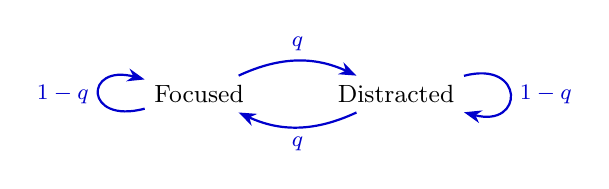
\begin{tikzpicture}[
                    every node/.style={font=\small},
                    every edge/.style={draw, thick, blue!80!black, -{Stealth[length=2.2mm]}}
                    ]
                    \node (F) at (0,0) {Focused};
                    \node (D) at (2.5,0) {Distracted};

                    % Transitions between states
                    \path (F) edge[bend left=25] node[above, font=\footnotesize, text=blue!80!black] {$q$} (D);
                    \path (D) edge[bend left=25] node[below, font=\footnotesize, text=blue!80!black] {$q$} (F);

                    % Self-loops
                    \path (F) edge[loop left, min distance=8mm] node[left, font=\footnotesize, text=blue!80!black] {$1-q$} (F);
                    \path (D) edge[loop right, min distance=8mm] node[right, font=\footnotesize, text=blue!80!black] {$1-q$} (D);
                \end{tikzpicture}
            }
        \end{column}

        \begin{column}{0.48\textwidth}
            \uncover<2->{
                \centering
                \textbf{\textcolor{teal!90!black}{Observation Model}}
                \vspace{0.6em}
                \begin{align*}
                    \textcolor{teal!90!black}{p(\text{Respond} \mid \text{Focused})}    & = \textcolor{teal!90!black}{0.9} \\
                    \textcolor{teal!90!black}{p(\text{Respond} \mid \text{Distracted})} & = \textcolor{teal!90!black}{0.5}
                \end{align*}
            }
        \end{column}
    \end{columns}

    \vspace{1.5em}

    % Row 2: Bottom two quadrants
    \begin{columns}[T,onlytextwidth]
        \begin{column}{0.48\textwidth}
            \uncover<3->{
                \centering
                \textbf{HMM/SSM}
                \vspace{0.8em}

                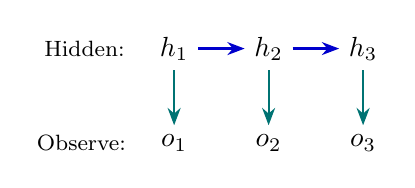
\begin{tikzpicture}[
                    every node/.style={font=\normalsize},
                    every edge/.style={draw, thick, -{Stealth[length=2.2mm]}}
                    ]
                    % Hidden states (latent)
                    \node (h1) at (0.6, 1.2) {$h_1$};
                    \node (h2) at (1.8, 1.2) {$h_2$};
                    \node (h3) at (3.0, 1.2) {$h_3$};

                    % Chain transitions (Transition Model: blue)
                    \path (h1) edge[draw=blue!80!black] (h2);
                    \path (h2) edge[draw=blue!80!black] (h3);

                    % Observations
                    \node (o1) at (0.6, 0) {$o_1$};
                    \node (o2) at (1.8, 0) {$o_2$};
                    \node (o3) at (3.0, 0) {$o_3$};

                    % Vertical emission arrows (Observation Model: teal)
                    \path (h1) edge[draw=teal!90!black] (o1);
                    \path (h2) edge[draw=teal!90!black] (o2);
                    \path (h3) edge[draw=teal!90!black] (o3);

                    % Labels on left
                    \node[left=0.2cm of h1, font=\footnotesize] {Hidden:};
                    \node[left=0.2cm of o1, font=\footnotesize] {Observe:};
                \end{tikzpicture}
            }
        \end{column}

        \begin{column}{0.48\textwidth}
            \uncover<4->{
                \centering
                \textbf{Belief state at time $t$}
                \vspace{1em}

                $b_t(h_t) := p(h_{t} \mid o_{1:t})$ all info for after $t$\\
                \vspace{0.3em}
                {\footnotesize $o_{1:t} = (o_1, o_2, \dots, o_t)$ is observation history.}
            }
        \end{column}
    \end{columns}
\end{frame}


% ------------------------------------------------------------------------------
\begin{frame}{Law of Total Probability \& Bayes' Rule}
    \textbf{Law of Total Probability}
    \begin{align*}
        P(A)                    & = \sum_{i} P(A \mid B_i) P(B_i)                           \\
        p(h_{t+1} \mid o_{1:t}) & = \int p(h_{t+1} \mid h_t) \, p(h_t \mid o_{1:t}) \, dh_t
    \end{align*}

    \vspace{0.4em}
    \hrule
    \vspace{0.6em}

    \textbf{Bayes' Rule}
    \begin{align*}
        P(A \mid B)               & = \frac{P(B \mid A) P(A)}{P(B)}                                                      \\
        p(h_{t+1} \mid o_{1:t+1}) & = \frac{p(o_{t+1} \mid h_{t+1}) \, p(h_{t+1} \mid o_{1:t})}{p(o_{t+1} \mid o_{1:t})}
    \end{align*}
\end{frame}


% ------------------------------------------------------------------------------
\begin{frame}{Recursive Bayesian Estimation}
    \centering
    % Transition arrow
    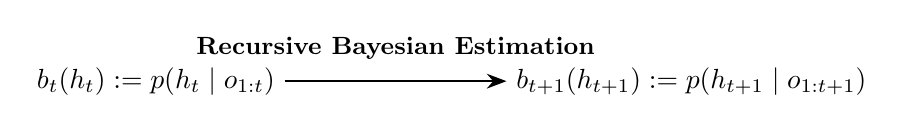
\begin{tikzpicture}[
        every node/.style={font=\normalsize},
        every edge/.style={draw, thick, -{Stealth[length=2.5mm]}}
        ]
        \node (curr) at (0, 0) {$b_t(h_t) := p(h_t \mid o_{1:t})$};
        \node (next) at (6.8, 0) {$b_{t+1}(h_{t+1}) := p(h_{t+1} \mid o_{1:t+1})$};

        \path (curr) edge node[above=0.15cm, font=\small\bfseries] {Recursive Bayesian Estimation} (next);
    \end{tikzpicture}

    \vspace{0.8em}

    \raggedright
    \textbf{1. Prediction Step} {\footnotesize (Law of Total Probability)}
    \[
        \overbrace{p(h_{t+1} \mid o_{1:t})}^{\text{Predicted Belief}} = \int \overbrace{\textcolor{blue!80!black}{p(h_{t+1} \mid h_t)}}^{\text{\textcolor{blue!80!black}{Transition Model}}} \, \underbrace{p(h_t \mid o_{1:t})}_{b_t(h_t)} \, dh_t
    \]

    \vspace{0.3em}

    \textbf{2. Update Step} {\footnotesize (Bayes' Rule)}
    \vspace{-1.8em}
    \begin{align*}
        b_{t+1}(h_{t+1}) = p(h_{t+1} \mid o_{1:t+1})
         & = \frac{\overbrace{\textcolor{teal!90!black}{p(o_{t+1} \mid h_{t+1})}}^{\text{\textcolor{teal!90!black}{Observation Model}}} \, p(h_{t+1} \mid o_{1:t})}{p(o_{t+1} \mid o_{1:t})} \\[0.5em]
         & = \frac{\textcolor{teal!90!black}{p(o_{t+1} \mid h_{t+1})} \, p(h_{t+1} \mid o_{1:t})}{\int \textcolor{teal!90!black}{p(o_{t+1} \mid h_{t+1})} \, p(h_{t+1} \mid o_{1:t}) \, dh_{t+1}}
    \end{align*}
\end{frame}
%
% ------------------------------------------------------------------------------
\begin{frame}{Belief Markov Chain}
    \centering
    \vspace{-0.4em}
    \textbf{$\{b_t\}$ is a Markov Chain:}
    \vspace{-0.7em}
    \[
        p(b_{t+1} \mid b_t, b_{t-1}, \dots, b_0) = p(b_{t+1} \mid b_t)
    \]

    \vspace{-0.2em}
    % Branching diagram
    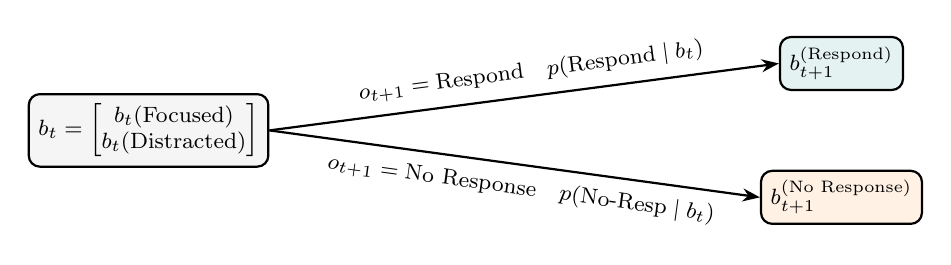
\begin{tikzpicture}[
        every node/.style={font=\footnotesize},
        box/.style={draw, rounded corners, thick, inner sep=3.5pt, align=center, fill=gray!8},
        arrow/.style={draw, thick, -{Stealth[length=2.2mm]}}
        ]
        % Root: Current belief
        \node[box] (root) at (-2.2, 0) {$b_t = \begin{bmatrix} b_t(\text{Focused}) \\ b_t(\text{Distracted}) \end{bmatrix}$};

        % Branches
        \node[box, fill=teal!10] (up) at (6.6, 0.85) {$b_{t+1}^{(\text{Respond})}$};
        \node[box, fill=orange!10] (down) at (6.6, -0.85) {$b_{t+1}^{(\text{No Response})}$};

        % Edges with transition probabilities
        \path (root.east) edge[arrow] node[above=1pt, pos=0.52, sloped] {$o_{t+1} = \text{Respond} \quad p(\text{Respond} \mid b_t)$} (up.west);
        \path (root.east) edge[arrow] node[below=1pt, pos=0.52, sloped] {$o_{t+1} = \text{No Response} \quad p(\text{No-Resp} \mid b_t)$} (down.west);
    \end{tikzpicture}

    \vspace{0.4em}
    \hrule
    \vspace{0.4em}

    \[
        p(\text{Respond} \mid b_t) = \textcolor{teal!90!black}{0.9} \, p(h_{t+1} = \text{F} \mid b_t) + \textcolor{teal!90!black}{0.5} \, p(h_{t+1} = \text{D} \mid b_t)
    \]

    \vspace{0.2em}
    \raggedright
    \begin{itemize}
        \item Both branch probabilities and $b_{t+1}$ depend \textbf{only} on $b_t$.
        \item Observation history $o_{1:t}$ is \textbf{not needed}.
    \end{itemize}
\end{frame}
% ------------------------------------------------------------------------------
\begin{frame}{Fixed Hidden States}
    % Row 1: Top two quadrants
    \begin{columns}[T,onlytextwidth]
        \begin{column}{0.48\textwidth}
            \uncover<1->{
                \centering
                \textbf{\textcolor{blue!80!black}{Prior Distribution}}
                \vspace{0.6em}
                \begin{align*}
                    \textcolor{blue!80!black}{q} & = \textcolor{blue!80!black}{0} \\
                    \textcolor{blue!80!black}{p(h = \text{Distracted})} & = \textcolor{blue!80!black}{0.2} \\
                    \textcolor{blue!80!black}{p(h = \text{Focused})}    & = \textcolor{blue!80!black}{0.8}
                \end{align*}
            }
        \end{column}

        \begin{column}{0.48\textwidth}
            \uncover<2->{
                \centering
                \textbf{\textcolor{teal!90!black}{Observation Model}}
                \vspace{0.6em}
                \begin{align*}
                    \textcolor{teal!90!black}{p(\text{Respond} \mid \text{Focused})}    & = \textcolor{teal!90!black}{0.9} \\
                    \textcolor{teal!90!black}{p(\text{Respond} \mid \text{Distracted})} & = \textcolor{teal!90!black}{0.5}
                \end{align*}
            }
        \end{column}
    \end{columns}

    \vspace{1.5em}

    % Row 2: Bottom two quadrants
    \begin{columns}[T,onlytextwidth]
        \begin{column}{0.48\textwidth}
            \uncover<3->{
                \centering
                \textbf{Fixed State Model}
                \vspace{0.8em}

                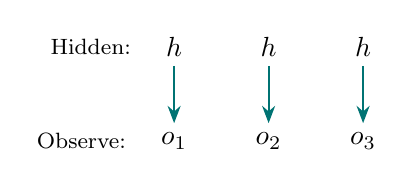
\begin{tikzpicture}[
                    every node/.style={font=\normalsize},
                    every edge/.style={draw, thick, -{Stealth[length=2.2mm]}}
                    ]
                    % Hidden state (fixed latent, no transitions)
                    \node (h1) at (0.6, 1.2) {$h$};
                    \node (h2) at (1.8, 1.2) {$h$};
                    \node (h3) at (3.0, 1.2) {$h$};

                    % Observations
                    \node (o1) at (0.6, 0) {$o_1$};
                    \node (o2) at (1.8, 0) {$o_2$};
                    \node (o3) at (3.0, 0) {$o_3$};

                    % Vertical emission arrows (Observation Model: teal)
                    \path (h1) edge[draw=teal!90!black] (o1);
                    \path (h2) edge[draw=teal!90!black] (o2);
                    \path (h3) edge[draw=teal!90!black] (o3);

                    % Labels on left
                    \node[left=0.2cm of h1, font=\footnotesize] {Hidden:};
                    \node[left=0.2cm of o1, font=\footnotesize] {Observe:};
                \end{tikzpicture}
            }
        \end{column}

        \begin{column}{0.48\textwidth}
            \uncover<4->{
                \centering
                \textbf{Belief state at time $t$}
                \vspace{1em}

                $b_t(h) := p(h \mid o_{1:t})$ all info for after $t$\\
                \vspace{0.3em}
                {\footnotesize $o_{1:t} = (o_1, o_2, \dots, o_t)$ is observation history.}
            }
        \end{column}
    \end{columns}
\end{frame}


% ------------------------------------------------------------------------------
\begin{frame}{Delayed Observations \& State Augmentation}
    \begin{columns}[T,onlytextwidth]
        \begin{column}{0.48\textwidth}
            \centering
            \textbf{Delayed Observation}
            \vspace{0.4em}

            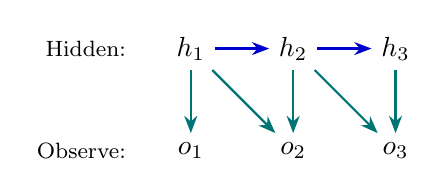
\begin{tikzpicture}[
                every node/.style={font=\normalsize},
                every edge/.style={draw, thick, -{Stealth[length=2.2mm]}}
                ]
                % Labels on left
                \node[anchor=east, font=\footnotesize] at (0.2, 1.3) {Hidden:};
                \node[anchor=east, font=\footnotesize] at (0.2, 0.0) {Observe:};

                % Hidden states
                \node (h1) at (0.9, 1.3) {$h_1$};
                \node (h2) at (2.2, 1.3) {$h_2$};
                \node (h3) at (3.5, 1.3) {$h_3$};

                % Chain transitions
                \path (h1) edge[draw=blue!80!black] (h2);
                \path (h2) edge[draw=blue!80!black] (h3);

                % Observations
                \node (o1) at (0.9, 0.0) {$o_1$};
                \node (o2) at (2.2, 0.0) {$o_2$};
                \node (o3) at (3.5, 0.0) {$o_3$};

                % Emission arrows: ht -> ot
                \path (h1) edge[draw=teal!90!black] (o1);
                \path (h2) edge[draw=teal!90!black] (o2);
                \path (h3) edge[draw=teal!90!black] (o3);

                % Delayed emission arrows: ht-1 -> ot
                \path (h1) edge[draw=teal!90!black] (o2);
                \path (h2) edge[draw=teal!90!black] (o3);
            \end{tikzpicture}

            \vspace{0.6em}
            \raggedright
            \begin{itemize}
                \item Memory in observation:
                \[
                    o_t \sim \textcolor{teal!90!black}{p(o_t \mid h_t, h_{t-1})}
                \]
                \item Breaks standard 1-step emission.
            \end{itemize}
        \end{column}

        \begin{column}{0.48\textwidth}
            \centering
            \textbf{State Augmentation}
            \vspace{0.4em}

            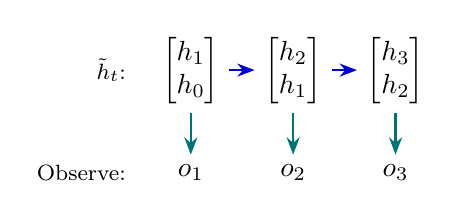
\begin{tikzpicture}[
                every node/.style={font=\normalsize},
                every edge/.style={draw, thick, -{Stealth[length=2.2mm]}}
                ]
                % Labels on left
                \node[anchor=east, font=\footnotesize] at (0.2, 1.3) {$\tilde{h}_t$:};
                \node[anchor=east, font=\footnotesize] at (0.2, 0.0) {Observe:};

                % Stacked hidden states
                \node (s1) at (0.9, 1.3) {$\begin{bmatrix} h_1 \\ h_0 \end{bmatrix}$};
                \node (s2) at (2.2, 1.3) {$\begin{bmatrix} h_2 \\ h_1 \end{bmatrix}$};
                \node (s3) at (3.5, 1.3) {$\begin{bmatrix} h_3 \\ h_2 \end{bmatrix}$};

                % Transitions between augmented states
                \path (s1) edge[draw=blue!80!black] (s2);
                \path (s2) edge[draw=blue!80!black] (s3);

                % Observations
                \node (o1) at (0.9, 0.0) {$o_1$};
                \node (o2) at (2.2, 0.0) {$o_2$};
                \node (o3) at (3.5, 0.0) {$o_3$};

                % Single emission arrows from stacked state to ot
                \path (s1) edge[draw=teal!90!black] (o1);
                \path (s2) edge[draw=teal!90!black] (o2);
                \path (s3) edge[draw=teal!90!black] (o3);
            \end{tikzpicture}

            \vspace{0.6em}
            \raggedright
            \begin{itemize}
                \item Augmented state: $\tilde{h}_t \coloneqq \begin{bmatrix} h_t \\ h_{t-1} \end{bmatrix}$
                \[
                    o_t \sim \textcolor{teal!90!black}{p(o_t \mid \tilde{h}_t)}
                \]
                \item Recovers standard HMM/SSM.
            \end{itemize}
        \end{column}
    \end{columns}
\end{frame}
 

\begin{frame}{Partially Observable MDP (POMDP)}
    \centering
    \vspace{-0.2em}
    \textbf{POMDP = Partially Observable MDP}

    \vspace{0.6em}
    \begin{columns}[T,onlytextwidth]
        \begin{column}{0.44\textwidth}
            \centering
            \textbf{MDP + Hidden Markov Chain}
            \vspace{0.4em}
            \begin{itemize}
                \item State $h_t$ is hidden.
                \item Hidden MC:
                \vspace{-0.3em}
                \[
                    h_{t+1} \sim p(h_{t+1} \mid h_t, a_t)
                \]
                \item $o_t$ is not Markovian:
                \vspace{-0.3em}
                \[
                    p(o_{t+1} \mid o_{1:t}) \ne p(o_{t+1} \mid o_t)
                \]
            \end{itemize}
        \end{column}
        \begin{column}{0.08\textwidth}
            \centering
            \vspace{5.5em}
            {\Large $\longrightarrow$}
        \end{column}
        \begin{column}{0.46\textwidth}
            \centering
            \textbf{MDP + Belief MC}
            \vspace{0.4em}
            \begin{itemize}
                \item Belief state $b_t(h_t) = p(h_t \mid o_{1:t})$.
                \item $\{b_t\}$ is a Markov Chain (RBE).
                \item MDP on beliefs:
                \vspace{-0.5em}
                \[
                    b_{t+1} = \tau(b_t, a_t, o_{t+1})
                \]
                \item Reward: $\rho(b_t, a_t) = \mathbb{E}_{h_t \sim b_t}[r_t(h_t, a_t)]$.
            \end{itemize}
        \end{column}
    \end{columns}
\end{frame}

% ------------------------------------------------------------------------------
\begin{frame}{Bayesian Bandit: Worker Selection}
    \begin{columns}[T,onlytextwidth]
        \begin{column}{0.48\textwidth}
            \textbf{2 Workers ($i \in \{1, 2\}$)}
            \begin{itemize}
                \item Fixed state: $h^{(i)} \in \{\text{Focused}, \text{Distracted}\}$
                \item Prior: $p(h^{(i)} = \text{Focused}) = 0.5$
                \item Action: hire worker $a_t \in \{1, 2\}$
            \end{itemize}
        \end{column}

        \begin{column}{0.48\textwidth}
            \textbf{Observation ($o_t \in \{0, 1\}$)}
            \begin{itemize}
                \item $p(o_t = 1 \mid \text{Focused}) = 0.9$
                \item $p(o_t = 1 \mid \text{Distracted}) = 0.5$
                \item Unhired worker provides no observation
            \end{itemize}
        \end{column}
    \end{columns}

    \vspace{0.6em}
    \hrule
    \vspace{0.6em}

    \textbf{Belief MDP}
    \begin{itemize}
        \item State: continuous belief $b_t = (b_t^{(1)}, b_t^{(2)}) \in [0, 1]^2$.
        \item Bayes-optimal via Value Iteration:
        \[
            V^*(b) = \max_{a} \Big\{ \rho(b, a) + \gamma \sum_o p(o \mid b, a) \, V^*(\tau(b, a, o)) \Big\}
        \]
        \vspace{-1.5em}
        \item \textbf{Bottleneck}: coupled continuous DP is intractable for large $K$.
        \item \textbf{Gittins Index} (summer school): decouples into 1D indices for each worker!
    \end{itemize}
\end{frame}

% ------------------------------------------------------------------------------
\begin{frame}{Duality: Stochastic vs.\ Bayesian Bandits}
    \begin{columns}[T,onlytextwidth]
        \begin{column}{0.48\textwidth}
            \textbf{Stochastic (Frequentist)}
            \begin{itemize}
                \item Fixed environment $\nu \in \mathcal{E}$.
                \item Minimax regret:
                \vspace{-0.4em}
                \[
                    R_n^*(\mathcal{E}) = \inf_{\pi} \sup_{\nu \in \mathcal{E}} R_n(\pi, \nu)
                \]
            \end{itemize}
        \end{column}

        \begin{column}{0.48\textwidth}
            \textbf{Bayesian}
            \begin{itemize}
                \item Prior $Q \in \Delta(\mathcal{E})$: $\nu \sim Q$.
                \item Bayesian regret:
                \vspace{-0.4em}
                \[
                    \mathrm{BR}_n(\pi, Q) = \mathbb{E}_{\nu \sim Q} [R_n(\pi, \nu)]
                \]
            \end{itemize}
        \end{column}
    \end{columns}

    \vspace{0.3em}
    \hrule
    \vspace{0.3em}

    \textbf{Minimax Duality via Sion's Theorem}
    \begin{itemize}
        \item Regret is convex in policy $\pi$ and linear in prior distribution $Q$.
        \item \textbf{Sion's minimax theorem} (compact $\mathcal{E}$) allows swapping $\inf$ and $\sup$:
        \vspace{-0.4em}
        \[
            \inf_{\pi} \sup_{\nu \in \mathcal{E}} R_n(\pi, \nu)
            = \sup_{Q \in \Delta(\mathcal{E})} \inf_{\pi} \mathrm{BR}_n(\pi, Q)
        \]
        \vspace{-0.6em}
        \item \textbf{Duality}: Minimax regret equals Bayes regret under worst-case prior $Q^*$.
        \item Frequentist minimax lower bounds can be proved via Bayesian priors!
    \end{itemize}

    \vspace{0.2em}
    {\tiny \textcolor{gray}{Reference: \cite{lattimore_bandit_2020}}}
\end{frame}
% ------------------------------------------------------------------------------
\begin{frame}{Imperfect-Information Games $\to$ Belief Games \& POMDPs}
    \begin{columns}[T,onlytextwidth]
        \begin{column}{0.48\textwidth}
            \textbf{Imperfect Info (e.g., Poker)}
            \begin{itemize}
                \item Hidden private states (cards).
                \item Actions leak private info; subgame solving must balance across hands.
            \end{itemize}
        \end{column}

        \begin{column}{0.48\textwidth}
            \textbf{Public Belief State (PBS)}
            \begin{itemize}
                \item Public history is common knowledge.
                \item Joint belief $\beta \in \Delta(\mathcal{S}_1 \times \mathcal{S}_2)$.
                \item Yields \textbf{perfect-information game} on belief states (Brown et al., ReBeL).
            \end{itemize}
        \end{column}
    \end{columns}

    \vspace{0.3em}
    \hrule
    \vspace{0.25em}

    \textbf{Reduction to POMDP (Known Opponent Strategy)}
    \begin{itemize}
        \item If opponent policy $\pi_{-i}$ is \textbf{fixed/known}, it is absorbed into dynamics:
        \vspace{-0.45em}
        \[
            p(s', o \mid s, a_i) = \sum_{a_{-i}} \pi_{-i}(a_{-i} \mid s, a_i) \, p(s', o \mid s, a_i, a_{-i})
        \]
        \vspace{-0.65em}
        \item Equilibrium collapses to a \textbf{single-agent POMDP} (Belief MDP).
    \end{itemize}

    \vspace{0.1em}
    {\tiny \textcolor{gray}{Reference: \cite{london_machine_learning_meetup_noam_2021}}}
\end{frame}

% ------------------------------------------------------------------------------
\begin{frame}{From Discrete Bandits to Continuous Domains}
    \begin{columns}[T,onlytextwidth]
        \begin{column}{0.48\textwidth}
            \textbf{\textcolor{blue!80!black}{Discrete Multi-Armed Bandit}}
            \begin{itemize}
                \item Finite action set $a \in \{1, \dots, K\}$.
                \item Independent reward distributions.
                \item Belief: posterior statistics per arm.
                \item Fails on continuous domains $\mathcal{X} \subset \mathbb{R}^d$.
            \end{itemize}
        \end{column}

        \begin{column}{0.48\textwidth}
            \textbf{\textcolor{teal!90!black}{Continuous Black-Box Setting}}
            \begin{itemize}
                \item Continuous domain $\mathcal{X} \subset \mathbb{R}^d$ ($\infty$ arms).
                \item Objective: $\max_{x \in \mathcal{X}} f(x)$ with costly $f$.
                \item Correlated: $x \approx x' \implies f(x) \approx f(x')$.
                \item \textbf{Latent state}: the unknown function $f$.
            \end{itemize}
        \end{column}
    \end{columns}

    \vspace{0.3em}
    \hrule
    \vspace{0.25em}

    \textbf{From Scalar Beliefs to Function Distributions}
    \begin{itemize}
        \item We need a prior distribution over an infinite-dimensional space $\mathcal{F}$.
        \item Closed-form recursive Bayesian conditioning $\implies$ \textbf{Gaussian Processes}!
    \end{itemize}
\end{frame}

% ------------------------------------------------------------------------------
\begin{frame}{Gaussian Processes: Priors over Functions}
    \begin{columns}[T,onlytextwidth]
        \begin{column}{0.48\textwidth}
            \textbf{\textcolor{blue!80!black}{Definition: $f \sim \mathcal{GP}(m, k)$}}
            \begin{itemize}
                \item Collection of random variables, any finite subset is jointly Gaussian:
                \vspace{-0.3em}
                \[
                    [f(x_1), \dots, f(x_n)]^\top \sim \mathcal{N}(\mathbf{m}, \mathbf{K})
                \]
                \vspace{-0.5em}
                \item Mean: $m(x) = \mathbb{E}[f(x)]$ (often $0$).
                \item Covariance: $\mathbf{K}_{ij} = k(x_i, x_j)$.
            \end{itemize}
        \end{column}

        \begin{column}{0.48\textwidth}
            \textbf{\textcolor{teal!90!black}{Covariance Kernel $k(x, x')$}}
            \begin{itemize}
                \item Encodes spatial correlation:
                \vspace{-0.3em}
                \[
                    k(x, x') = \mathrm{Cov}(f(x), f(x'))
                \]
                \vspace{-0.5em}
                \item \textbf{Squared Exponential (RBF)}:
                \vspace{-0.3em}
                \[
                    k(x, x') = \sigma_f^2 \exp\Big(-\frac{\|x - x'\|^2}{2\ell^2}\Big)
                \]
                \vspace{-0.5em}
                \item Lengthscale $\ell$: smoothness / reach.
            \end{itemize}
        \end{column}
    \end{columns}

    \vspace{0.3em}
    \hrule
    \vspace{0.25em}

    \textbf{Nonparametric Prior}: Instead of parameterizing $f(x; \mathbf{w})$, a GP directly specifies a consistent prior over the infinite-dimensional function space.
\end{frame}

% ------------------------------------------------------------------------------
\begin{frame}{Gaussian Conditioning: Exact Belief Updating}
    Given observations $\mathcal{D}_t = \{(x_i, y_i)\}_{i=1}^t$ with $y_i = f(x_i) + \varepsilon_i$, $\varepsilon_i \sim \mathcal{N}(0, \sigma_n^2)$:
    \vspace{-0.3em}
    \[
        \begin{pmatrix} \mathbf{y} \\ f(x^*) \end{pmatrix} \sim \mathcal{N}\left( \mathbf{0}, \begin{pmatrix} \mathbf{K} + \sigma_n^2 \mathbf{I} & \mathbf{k}_* \\ \mathbf{k}_*^\top & k(x^*, x^*) \end{pmatrix} \right)
    \]
    \vspace{-0.4em}
    \hrule
    \vspace{0.25em}

    \textbf{Exact Posterior Belief}: $f(x^*) \mid \mathcal{D}_t \sim \mathcal{N}(\mu_t(x^*), \sigma_t^2(x^*))$
    \vspace{-0.3em}
    \[
        \mu_t(x^*) = \mathbf{k}_*^\top (\mathbf{K} + \sigma_n^2 \mathbf{I})^{-1} \mathbf{y}, \qquad
        \sigma_t^2(x^*) = k(x^*, x^*) - \mathbf{k}_*^\top (\mathbf{K} + \sigma_n^2 \mathbf{I})^{-1} \mathbf{k}_*
    \]
    \vspace{-0.4em}

    \begin{columns}[T,onlytextwidth]
        \begin{column}{0.48\textwidth}
            \textbf{\textcolor{blue!80!black}{Exploitation: Mean $\mu_t(x^*)$}}
            \begin{itemize}
                \item Best estimate of function value.
                \item Interpolates data (smooths if $\sigma_n^2 > 0$).
            \end{itemize}
        \end{column}

        \begin{column}{0.48\textwidth}
            \textbf{\textcolor{teal!90!black}{Exploration: Variance $\sigma_t^2(x^*)$}}
            \begin{itemize}
                \item Quantifies \textbf{epistemic uncertainty}.
                \item Drops near samples; high in gaps.
            \end{itemize}
        \end{column}
    \end{columns}
\end{frame}

% ------------------------------------------------------------------------------
\begin{frame}{Bayesian Optimization: A POMDP over Function Space}
    \begin{columns}[T,onlytextwidth]
        \begin{column}{0.48\textwidth}
            \textbf{\textcolor{blue!80!black}{POMDP Elements}}
            \begin{itemize}
                \item \textbf{State} $s$: Unknown $f \sim \mathcal{GP}(0, k)$.
                \item \textbf{Action} $a_t$: Query point $x_t \in \mathcal{X}$.
                \item \textbf{Obs} $o_t$: $y_t = f(x_t) + \varepsilon_t$.
                \item \textbf{Belief} $b_t$: Posterior $\mathcal{GP}(\mu_t, \sigma_t^2)$.
            \end{itemize}
        \end{column}

        \begin{column}{0.48\textwidth}
            \textbf{\textcolor{teal!90!black}{Decision Regimes}}
            \begin{itemize}
                \item \textbf{Pure Exploration}: Terminal payoff at $T$.
                \item \textbf{Cumulative}: Reward at each step $t$.
                \item Exact belief update via GP conditioning.
            \end{itemize}
        \end{column}
    \end{columns}

    \vspace{0.25em}
    \hrule
    \vspace{0.25em}

    \begin{columns}[T,onlytextwidth]
        \begin{column}{0.48\textwidth}
            \textbf{Simple Regret (Pure Explore)}
            \vspace{-0.3em}
            \[
                S_T = \max\nolimits_{x \in \mathcal{X}} f(x) - f(\hat{x}_T)
            \]
            \vspace{-0.5em}
            \begin{itemize}
                \item Payoff only at final recommendation $\hat{x}_T$.
                \item E.g., hyperparameter tuning.
            \end{itemize}
        \end{column}

        \begin{column}{0.48\textwidth}
            \textbf{Cumulative Regret (Bandit)}
            \vspace{-0.3em}
            \[
                R_T = \sum\nolimits_{t=1}^T \big(\max\nolimits_x f(x) - f(x_t)\big)
            \]
            \vspace{-0.5em}
            \begin{itemize}
                \item Exploit during optimization.
                \item E.g., online routing, clinical trials.
            \end{itemize}
        \end{column}
    \end{columns}
\end{frame}

% ------------------------------------------------------------------------------
\begin{frame}[allowframebreaks]{References}
    \footnotesize
    \bibliographystyle{apalike}
    \nocite{*}
    \bibliography{references}
\end{frame}

\end{document}
